\section{Dynamiczny przydział priorytetów}
\label{ch:alg-priorities-allocation}
Obok samego algorytmu WHCA* zrealizowano własną metodę dynamicznego przydziału priorytetów oraz skalowania okna czasowego, która to przyczynia się do zwiększenia skuteczności planowania ruchu robotów. Stanowi ona niejako rozwinięcie metody WHCA* o dodatkowe procedury.
Dla rozróżnienia poszczególnych wariantów metody WHCA* w dalszej części pracy będziemy posługiwać się skrótowymi nazwami:
\begin{itemize}
	\item {\bf WHCA*1} - {\it Windowed Hierarchical Cooperative A*} bez dynamicznego przydzielania priorytetów, ze stałym oknem czasowym,
	\item {\bf WHCA*2} - {\it Windowed Hierarchical Cooperative A*} z dynamicznym przydziałem priorytetów, ze stałym oknem czasowym,
	\item {\bf WHCA*3} - {\it Windowed Hierarchical Cooperative A*} z dynamicznym przydziałem priorytetów oraz skalowaniem okna czasowego.
\end{itemize}

Układ priorytetów w metodzie WHCA* ma istotny wpływ na wynik planowania tras.
Priorytety robotów warunkują kolejność wyznaczania ich dróg.
Z tego powodu robot o wyższym priorytecie podczas planowania nie będzie uwzględniał agentów o priorytetach niższych, gdyż planowanie ich dróg odbywa się później.
Może to zatem spowodować wyznaczenie trasy kolizyjnej z robotem o niższym priorytecie.

\subsection{Detekcja kolizji}
Podobnie jak w algorytmie LRA*, również w metodzie WHCA* należy wykrywać kolizje (odpowiednio wcześniej).
Nawet w przypadku, gdy roboty podążają wzdłuż zaplanowanych ścieżek, wciąż istnieje możliwość wystąpienia kolizji.
Taka sytuacja może wystąpić, gdy robot, który planuje drogę wcześniej (ma wyższy priorytet), nie uwzględnia, że następnemu robotowi może nie udać się wyznaczenie trajektorii (z powodu właśnie zaplanowanej trasy).
Wykrywanie kolizji odbywa się tak samo, jak w przypadku metody LRA* (por. \ref{ch:alg-collision-avoid}).
Należy zaznaczyć, że pod pojęciem wykrywania kolizji rozumiemy wczesne zauważenie kolizji, która wystąpiłaby w następnym kroku. Niepożądane jest doprowadzanie do faktycznych kolizji, dlatego interwencja zachodzi odpowiednio wcześniej.

% TODO screen z przypadku kolizjii

\subsection{Wariant WHCA*2}
%TODO stała wartość okna
Wariant WHCA*2 został wzbogacony o dynamiczny przydział priorytetów agentów.
Zaproponowane podejście polega na zwiększaniu priorytetów robotów w przypadku niepowodzenia w znalezieniu trasy.
Opiera się to na następujących krokach:
\begin{enumerate}
	\item Początkowo roboty mają nadane priorytety losowo. Otrzymują kolejne wartości od 1 do liczby wszystkich robotów.
	\item Rozmiar okna czasowego jest zawsze równy całkowitej liczbie agentów zwiększonej o 1.
	\item Planowanie tras dla robotów wykonywane jest w przypadku detekcji kolizji w poprzednim kroku symulacji, lub gdy robot wykonał już wszystkie akcje z jego indywidualnej kolejki akcji.
	Lista robotów zostaje posortowana malejąco według priorytetów przed wykonaniem planowania tras. Wyższa wartość priorytetu oznacza pierwszeństwo podczas planowania.
	\item Następnie wykonywane jest planowanie tras zgodnie z aktualnym układem kolejności robotów (jak w wariancie WHCA*1). Wyznaczone ścieżki zaznaczane są kolejno w tablicy rezerwacji.
	\item Jeśli dla któregoś robota nie została znaleziona bezkolizyjna ścieżka, to następuje zwiększenie jego priorytetu o wartość 1. Taki awans priorytetów może nastąpić dla wielu robotów w jednym kroku symulacji.
	\item Dla wszystkich robotów dokonywana jest weryfikacja wystąpienia kolizji. W przypadku jej wykrycia, kolejka ruchów obydwu (lub więcej) robotów zostaje opróżniona.
	\item W następnych krokach symulacji zostanie podjęta próba ponownego poszukiwania tras dla robotów, u których wystąpiło niepowodzenie planowania lub została wykryta kolizja. Tym razem nastąpi to z nowym układem priorytetów.
\end{enumerate}

Algorytm przewiduje możliwość posiadania przez wiele robotów tych samych wartości priorytetów.
Kolejność planowania dla takich robotów zależy wtedy od zastosowanego algorytmu sortowania list. W obecnej implementacji kolejność ta pozostaje taka sama, jak sprzed wystąpienia awansu priorytetów.

Warto dodać, że w sytuacji przedstawionej na rysunku \ref{fig:whca-giveway} metoda WHCA*2 byłaby w stanie doprowadzić roboty do celu niezależnie od początkowego układu priorytetów.

W przypadku wykrycia kolizji wielu robotów zwiększenie priorytetu dokonywane jest dla robota o niższym priorytecie.
Może to jednak prowadzić do naprzemiennego zwiększania priorytetów robotów powtarzającego się w nieskończonym cyklu.
Taki przypadek ilustruje rysunek \ref{fig:whca2-head}.
Robot nr 2 (niebieski) posiada priorytet równy 2 i wyznacza trasę jako pierwszy. Nie uwzględnia on robota nr 1 (czerwonego), dlatego wyznacza drogę po linii prostej do swojego celu, która koliduje z robotem nr 1.
W wyniku wykrytej kolizji zwiększa się priorytet robota nr 1 do wartości 3 (w dwóch kolejnych krokach symulacji) i kolejność planowania tras robotów zostaje odwrócona.
Następnie zwiększany jest priorytet robota nr 2, co powoduje powstanie niekończącego się cyklu.
Okno czasowe jest zbyt małe, aby roboty uznały drogę "na około" jako korzystniejszą, gdyż wymaga to oddalenia się od celu.
\begin{figure}[H]
	\centering
		\subfloat[]{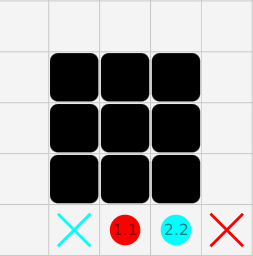
\includegraphics[width=0.3\columnwidth]{img/robopath/whca2-head-1}}
		\qquad
		\subfloat[]{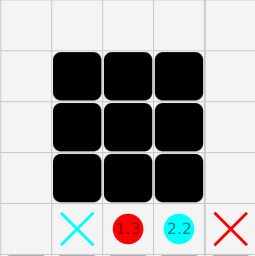
\includegraphics[width=0.3\columnwidth]{img/robopath/whca2-head-2}}
		\qquad
		\subfloat[]{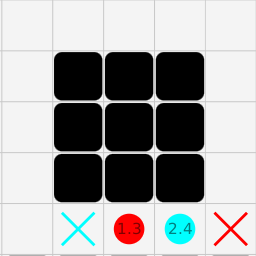
\includegraphics[width=0.3\columnwidth]{img/robopath/whca2-head-3}}
	\caption{Przykład cyklu naprzemiennego zwiększania priorytetów robotów uzyskanego metodą WHCA*2:
	(a) Robot nr 2 (niebieski) wyznacza trasę jako pierwszy, która koliduje z robotem nr 1 (czerownym).
	(b) Priorytet robota nr 1 zwiększa się do wartości 3.
	(c) Odwrócona kolejność planowania powoduje wzrost priorytetu robota nr 2.}
	\label{fig:whca2-head}
\end{figure}
Kolejny opisywany wariant WHCA*3 rozwiąże powyższy problem, wprowadzając w takich sytuacjach dodatkowe działanie.

\subsection{Wariant WHCA*3}
Wariant WHCA*3 stanowi rozszerzenie WHCA*2 o procedurę skalowania okna czasowego.
Rozmiar okna czasowego może zmieniać się w trakcie trwania symulacji.

Poniżej przedstawiono kroki wariantu WHCA*3. Modyfikacje w stosunku do wariantu WHCA*2 zostały w tekście wyróżnione (pogrubione). Wprowadzają one dodatkowe powiększanie okna czasowego do procedury dynamicznego przydziału priorytetów:
\begin{enumerate}
	\item Początkowo roboty mają nadane priorytety losowo. Otrzymują kolejne wartości od 1 do liczby wszystkich robotów.
	\item Rozmiar okna czasowego jest {\bf początkowo} równy całkowitej liczbie agentów zwiększonej o 1.
	\item Planowanie tras dla robotów wykonywane jest w przypadku detekcji kolizji w poprzednim kroku symulacji, lub gdy robot wykonał już wszystkie akcje z jego indywidualnej kolejki akcji.
	Lista robotów zostaje posortowana malejąco według priorytetów przed wykonaniem planowania tras. Wyższa wartość priorytetu oznacza pierwszeństwo podczas planowania.
	\item Następnie wykonywane jest planowanie tras zgodnie z aktualnym układem kolejności robotów (jak w wariancie WHCA*1). Wyznaczone ścieżki zaznaczane są kolejno w tablicy rezerwacji.
	\item Jeśli dla któregoś robota nie została znaleziona bezkolizyjna ścieżka, to następuje zwiększenie jego priorytetu o wartość 1. Taki awans priorytetów może nastąpić dla wielu robotów w jednym kroku symulacji.
	\begin{enumerate}
		\item {\bf Jeśli nowa wartość priorytetu robota przekracza aktualną wartość rozmiaru okna czasowego, to okno czasowe zostaje zwiększone do wartości równej maksymalnemu priorytetowi robota.}
	\end{enumerate}
	\item Dla wszystkich robotów dokonywana jest weryfikacja wystąpienia kolizji. W przypadku jej wykrycia, kolejka ruchów obydwu (lub więcej) robotów zostaje opróżniona.
	\item W następnych krokach symulacji zostanie podjęta próba ponownego poszukiwania tras dla robotów, u których wystąpiło niepowodzenie planowania lub została wykryta kolizja. Tym razem nastąpi to z nowym układem priorytetów.
\end{enumerate}

Rozszerzanie okna czasowego pozwala na poszukiwanie coraz bardziej skomplikowanych rozwiązań, gdy wciąż nie udaje się znaleźć rozwiązania. Jednocześnie nie przeznaczamy większej mocy obliczeniowej już na początku, gdy prawdopodobnie odbyłoby się planowanie w niepotrzebnie dużej głębi przeszukiwania.

Wariant WHCA*3 rozwiązuje w wielu przypadkach problem naprzemiennego, niekończącego się zwiększania priorytetów robotów.
Wraz ze wzrostem priorytetów zwiększa się okno czasowe i analizowane są bardziej skomplikowane rozwiązania.
Sytuację tą ilustruje rysunek \ref{fig:whca3-head}.
Warto zaznaczyć, że z tego typu problemem nie poradziła sobie metoda WHCA*2 (por. rys. \ref{fig:whca2-head}).
\begin{figure}[H]
	\centering
		\subfloat[]{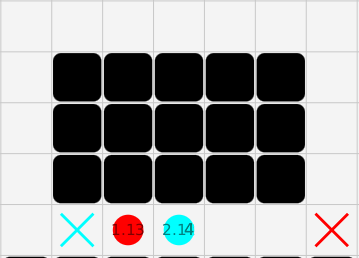
\includegraphics[width=0.3\columnwidth]{img/robopath/whca-head-4}}
		\qquad
		\subfloat[]{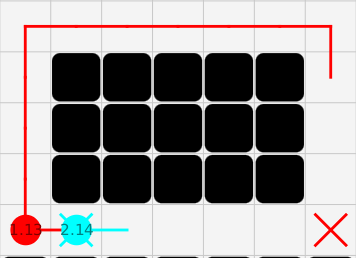
\includegraphics[width=0.3\columnwidth]{img/robopath/whca-head-5}}
		\qquad
		\subfloat[]{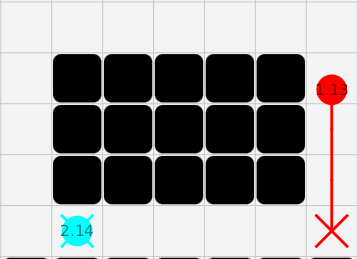
\includegraphics[width=0.3\columnwidth]{img/robopath/whca-head-6}}
	\caption{Przykład planowania tras metodą WHCA*3:
	(a) Priorytety robotów (oraz okno czasowe) wzrastają do wartości równej 14.
	(b) Wzrost rozmiaru okna czasowego powoduje odnalezienie alternatywnej drogi przez robota nr 1.
	(c) Po kolejnym planowaniu tras roboty osiągają punkty docelowe.}
	\label{fig:whca3-head}
\end{figure}

% TODO screeny ciekawych przypadków
% \begin{figure}
% 	\centering
% 	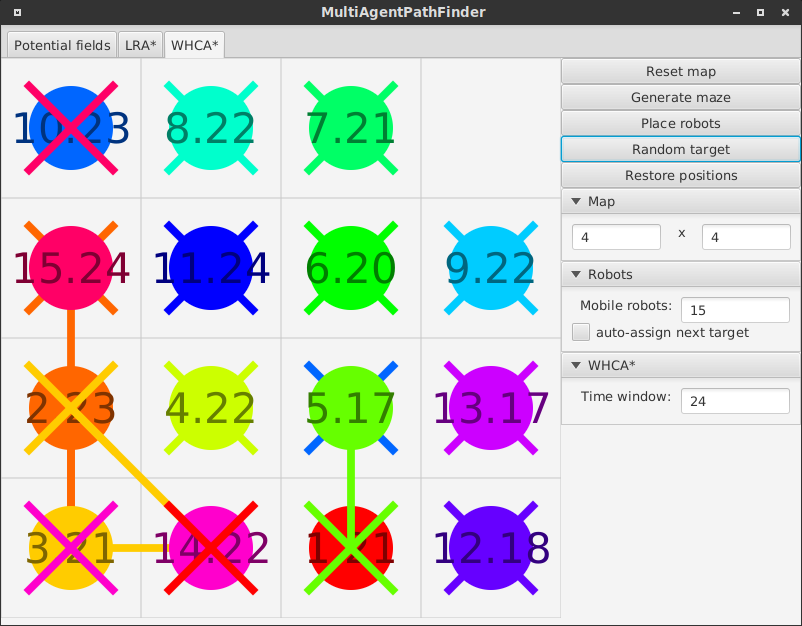
\includegraphics[width=0.8\columnwidth]{img/robopath/puzzle-15}
% 	\caption{Metoda WHCA*3: puzzle 15}
% 	\label{fig:test-puzzle-15}
% \end{figure}

Wykonane testy potwierdziły wzrost skuteczności w wyznaczaniu tras dzięki wprowadzeniu metody zarówno dynamicznego przydziału priorytetów jak i rozszerzania okna czasowego dla algorytmu WHCA* (por. \ref{ch:test-results}).